
\section{Tutorial of StartupBench Task Annotation}

\subsection{Task Construction}
\label{app:task_construction}

A \textsc{startup} task can be defined as a triple $\mathcal{T}=(q,\mathcal{E},\mathcal{R})$.
The experts are required to provide all the elements of a task:

\begin{itemize}
    \item \textbf{Input query}: The query $q$ is a natural-language statement of the task, specifying the user instruction that initiates the task. Derived from authentic scenarios of the work of annotators, the input query is supposed to reflect realistic user intent, including task background, implicit constraints and expected deliverables.

    \item \textbf{Task workspace}: The environment $\mathcal{E}$ denotes the complete workspace provided to the agent, including the multimodal source files together with any additional resources and interaction setting required to complete the task. The task workspace provides a self-contained execution environment for the agent. Each workspace includes all necessary input artifacts (e.g., files, datasets, or structured resources) required to complete the task, and ensures that the agent has access to sufficient input information to solve the problem. This design enables reproducible evaluation under controlled conditions while preserving realistic workflow structure.

    \item \textbf{Evaluation rubrics}: The rubric $\mathcal{R}=\{(p_i,w_i)\}_{i=1}^{n}$ is a checklist within which every item consists of a natural-language scoring point $p_i$ and a positive importance weight $w_i$ reflecting its importance to successful task completion. The evaluation rubrics define a set of fine-grained criteria used to assess task completion quality. Due to the complexity and multi-faceted nature of real-world workflows, each task is evaluated using multiple rubric items covering different dimensions. We categorize all rubrics in StartupBench into 6 dimensions and 3 importance levels, which are detailed in Appendix~\ref{app:rubrics}.

\end{itemize}

Together, these components preserve the structure of real-world agent workflows while enabling systematic and objective evaluation. Tasks may require information synthesis, constraint following, structured generation, or domain-specific reasoning and judgment.


\subsection{Cross Validation}
\label{app:cross_valid}


To ensure reliability of the quality of data, in our construction process each task is independently reviewed by at least one additional domain expert with relevant professional experience. Rather than focusing only on annotation consistency, reviewers validate the realism and correctness of the task from multiple complementary perspectives.

\begin{itemize} \item \textbf{Task authenticity.} Reviewers verify the authenticity of both the task description and the accompanying workspace. This includes checking that the input query reflects realistic user requests, that all provided materials are factually correct, and that no domain-specific knowledge errors exist.

\item \textbf{Workflow fidelity.} Reviewers examine whether the task faithfully represents real-world workflows in the corresponding profession. Tasks that deviate from practical working procedures or fail to reflect genuine job responsibilities are revised or discarded.

\item \textbf{Rubric validity.} Reviewers inspect the evaluation rubrics to ensure that the assessed capabilities are meaningful for the target workflow, that rubric items are clear and unambiguous, and that their relative weights reasonably reflect task priorities.

\item \textbf{Ground-truth verification.} Reviewers validate the reference solution (ground truth) by evaluating it against the finalized rubrics. The ground-truth deliverable is required to achieve a full score. If inconsistencies are identified between the reference solution and the evaluation criteria, both the solution and the rubrics are revised until they are mutually consistent. \end{itemize}

\section{Domain Expert Background}
\label{app:expert background}
We recruit 57 domain experts to support task construction and cross-validation. The expert pool covers all 6 domains in StartupBench and spans a diverse range of professional backgrounds, including clinical medicine, law, investment and quantitative finance, software development and artificial intelligence, engineering, business management and consulting, and education and humanities. Experts are assigned to tasks according to their reported areas of expertise and professional experience, ensuring that task construction and review were conducted by individuals familiar with the corresponding professional domains.

Table~\ref{tab:expert_background} summarizes the professional experience of the expert pool. The median professional experience is 5 years. Among the 57 experts, 68.4\% have at least 3 years of professional experience, 42.1\% have at least 6 years, and 24.6\% have at least 10 years. These backgrounds provide practical domain knowledge for translating interview-derived user scenarios into reproducible benchmark tasks and for assessing the realism, correctness, and evaluation criteria of tasks during cross-validation. All experts are reasonably compensated based on the actual workload associated with task construction and review.

\begin{table}[t]
\centering
\small
\caption{Summary of domain expert backgrounds. Professional experience refers to reported years of experience in the corresponding or closely related domain.}
\label{tab:expert_background}
\begin{tabular}{lc}
\toprule
\textbf{Expert Statistics} & \textbf{Value} \\
\midrule
Number of domain experts                  & 57    \\
Median professional experience            & 5 years \\
Experts with $\geq 3$ years of experience & 68.4\% \\
Experts with $\geq 6$ years of experience & 42.1\% \\
Experts with $\geq 10$ years of experience & 24.6\% \\
StartupBench domain coverage              & 6 / 6 \\
\bottomrule
\end{tabular}
\end{table}

\section{Rubrics of StartupBench}
\label{app:rubrics}


\textbf{Rubric Dimensions.} To facilitate consistent evaluation across heterogeneous real-world tasks, we organize all evaluation rubrics into six high-level categories according to the primary capability they assess. Rather than being tied to specific application domains, these categories capture common dimensions of deliverable quality that recur across office tasks, including correctness, completeness, data processing, professional reasoning, engineering quality, and presentation. This taxonomy enables more interpretable analysis of model strengths and weaknesses while maintaining a unified evaluation framework across different task types.

\begin{itemize}
    \item \textbf{Structure \& Completeness.}
    Evaluates whether the required deliverables are fully produced with the correct organization, file structure, required components, and overall completeness.

    \item \textbf{Calculation Precision.}
    Evaluates the correctness of numerical results, logical reasoning, formula execution, factual consistency, and other objective computations.

    \item \textbf{Information Integration.}
    Evaluates data cleaning, transformation, aggregation, statistical analysis, feature engineering, modeling, and other structured data manipulation workflows.

    \item \textbf{Domain-Specific Compliance.}
    Evaluates whether outputs satisfy domain-specific professional requirements, including business logic, financial principles, legal reasoning, medical practice, educational standards, and other expert knowledge.

    \item \textbf{Engineering \& Format.}
    Evaluates implementation quality, coding conventions, spreadsheet engineering, document formatting, reproducibility, robustness, naming conventions, and compliance with technical specifications.

    \item \textbf{Output \& Presentation.}
    Evaluates the quality of visual presentation and communication, including charts, layouts, formatting, readability, report organization, and overall usability of the final deliverables.
\end{itemize}

Table~\ref{tab:rubric_distribution} summarizes the distribution of all 2,453 rubrics in StartupBench.  Calculation Precision constitutes the largest rubric category (38.9\%), reflecting the importance of producing objectively correct work products. Structure \& Completeness and Domain-Specific Compliance together account for another 42.8\%, highlighting that successful completion of realistic office workflows requires not only correct computations but also complete deliverables and professional domain reasoning.

\begin{table}[h]
\centering
\small
\caption{Distribution of rubric categories in StartupBench.}
\label{tab:rubric_distribution}
\begin{tabular}{lc}
\toprule
\textbf{Category} & \textbf{Percentage} \\
\midrule
Structure \& Completeness & 27.31\% \\
Calculation Precision & 38.89\% \\
Information Integration & 9.46\% \\
Domain-Specific Compliance & 15.49\% \\
Engineering \& Format & 6.20\% \\
Output \& Presentation & 2.65\% \\
\midrule
\textbf{Total} & \textbf{100.00\%} \\
\bottomrule
\end{tabular}
\end{table}



\textbf{Rubric Importance Levels.} To account for differences in the importance of individual requirements to successful task completion, we assign each rubric to one of three importance levels. \textbf{Core} rubrics capture requirements that directly determine whether the primary user needs are satisfied; violating them would substantially compromise the correctness, reliability, safety, or usability of the final deliverable. \textbf{Important} rubrics represent key requirements for high-quality task completion whose satisfaction materially affects the overall quality of the deliverable, but whose individual violation does not necessarily render it unusable. \textbf{Auxiliary} rubrics capture lower-level requirements whose omission primarily affects details, user experience, visual appeal, or polish rather than the fundamental usability of the deliverable. We assign weights of \textbf{5}, \textbf{3}, and \textbf{1} to Core, Important, and Auxiliary rubrics, respectively, and use these weights when aggregating rubric-level judgments into the task score. A typical case of task containing rubrics of different levels is shown at Figure~\ref{fig:rubric_level}.

\begin{figure*}[t]
    \centering
    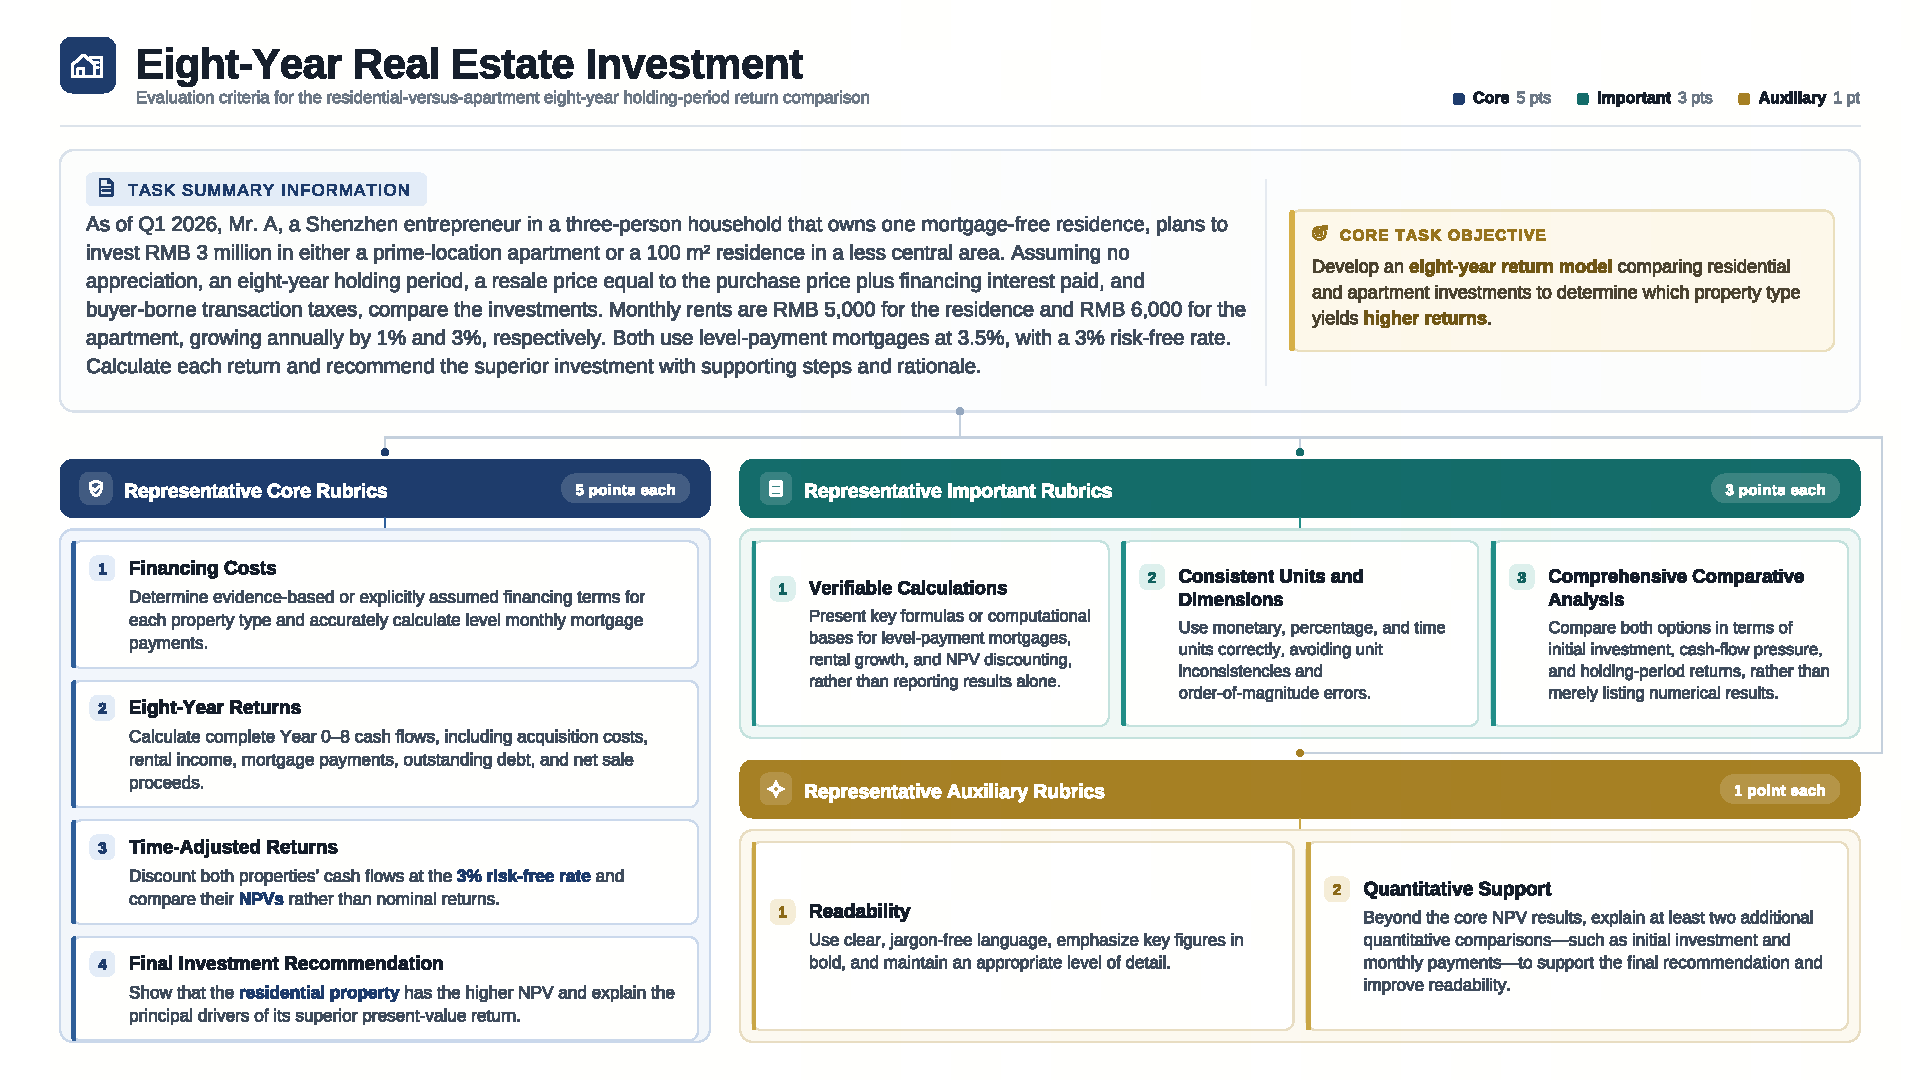
\includegraphics[width=0.99\textwidth]{figures/multi_level_rubric.pdf}
    \caption{
A representative example of a rubric of a task spanning 3 levels. Core rubrics assess the essential financial reasoning and calculations required to solve the investment problem, Important rubrics evaluate the correctness and completeness of the supporting analysis, while Auxiliary rubrics capture presentation quality and additional quantitative support.}
    \label{fig:rubric_level}
% \vspace{-6pt}
\end{figure*}

Across  all tasks, Core, Important, and Auxiliary rubrics account for an average of 59.10\%, 34.33\%, and 6.57\% of the total task weight, respectively, ensuring that task scores are primarily determined by requirements that materially affect successful task completion.




\section{Examples of Behavior-level Failure Modes}

\subsection{Self-Verification Hallucination}
\label{app:self-verify hallucination}

A representative example is shown in Fig.~\ref{fig:self_verify}. The task requires the model to filter all level-11 members, simulate route check-ins until each member reaches the level-12 threshold, and generate an Excel workbook satisfying a set of precise value and formatting constraints. The produced workbook appears largely complete, containing the required worksheet, member records, and output columns, leading the model to conclude that the task has been successfully finished. However, artifact-level inspection reveals multiple acceptance-critical errors, including incorrect effective-point values and mismatched member names. The underlying issue is not that the model fails to perform the required computation, but that it never verifies the generated artifact itself. Instead, it treats a successful execution summary as evidence that the final deliverable has been validated. Consequently, localized yet user-critical errors remain unnoticed, illustrating a form of \emph{self-verification hallucination}, where confidence is derived from the reasoning process rather than from independently checking the completed artifact against the original task requirements.

\begin{figure*}[t]
    \centering
    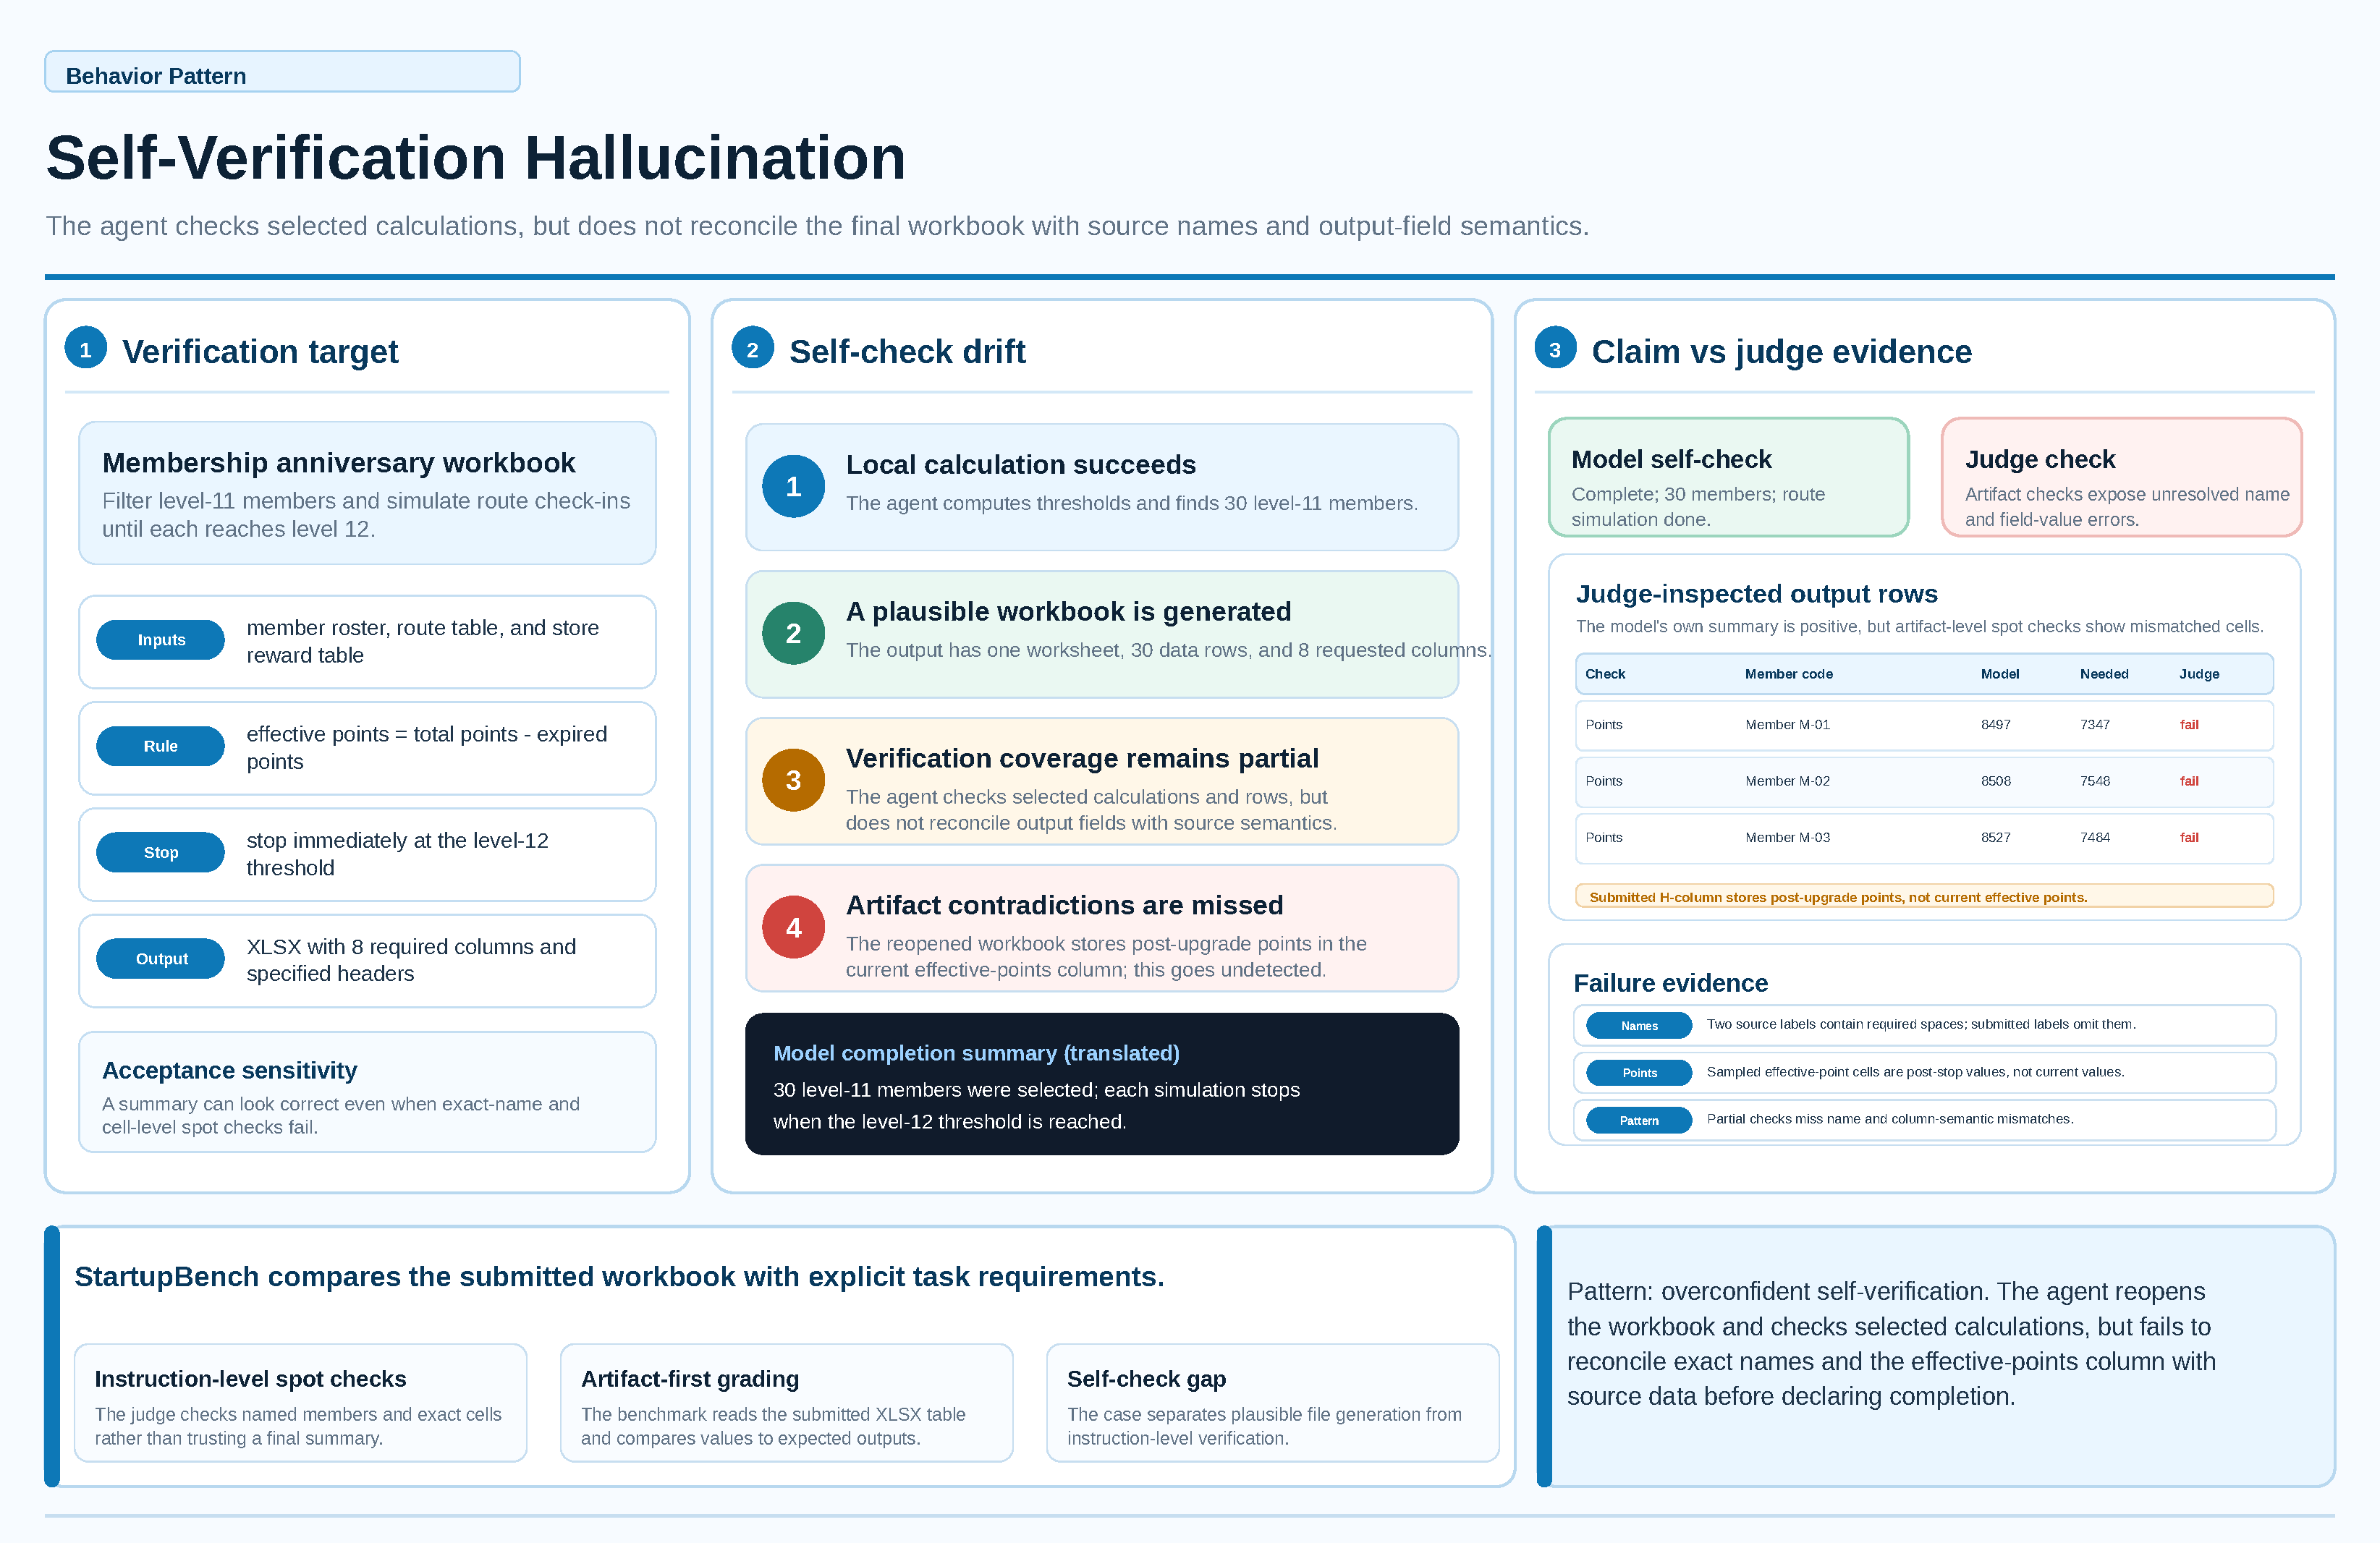
\includegraphics[width=0.99\textwidth]{figures/figure6_self_verification_hallucination.pdf}
    \caption{
A representative example of self-verification hallucination. The model generates a plausible workbook and concludes that the task has been completed based on its execution process. However, artifact-level spot checks expose acceptance-critical errors in the final deliverable, showing that the model mistakes a progress summary for actual verification instead of validating the generated artifact against the original task requirements.}
    \label{fig:self_verify}
% \vspace{-6pt}
\end{figure*}




\subsection{Domain-Specific Failure}
\label{app:domain}

A representative example of failure caused by insufficient domain-specific clinical actionability is shown at Figure~\ref{fig:domain-specify}. The model generates a well-formatted multidisciplinary treatment plan that appears clinically professional, yet violates multiple safety-critical treatment constraints. The failure stems not from poor writing quality, but from an inability to convert medical knowledge into actionable and clinically reliable decisions.

\begin{figure*}[t]
    \centering
    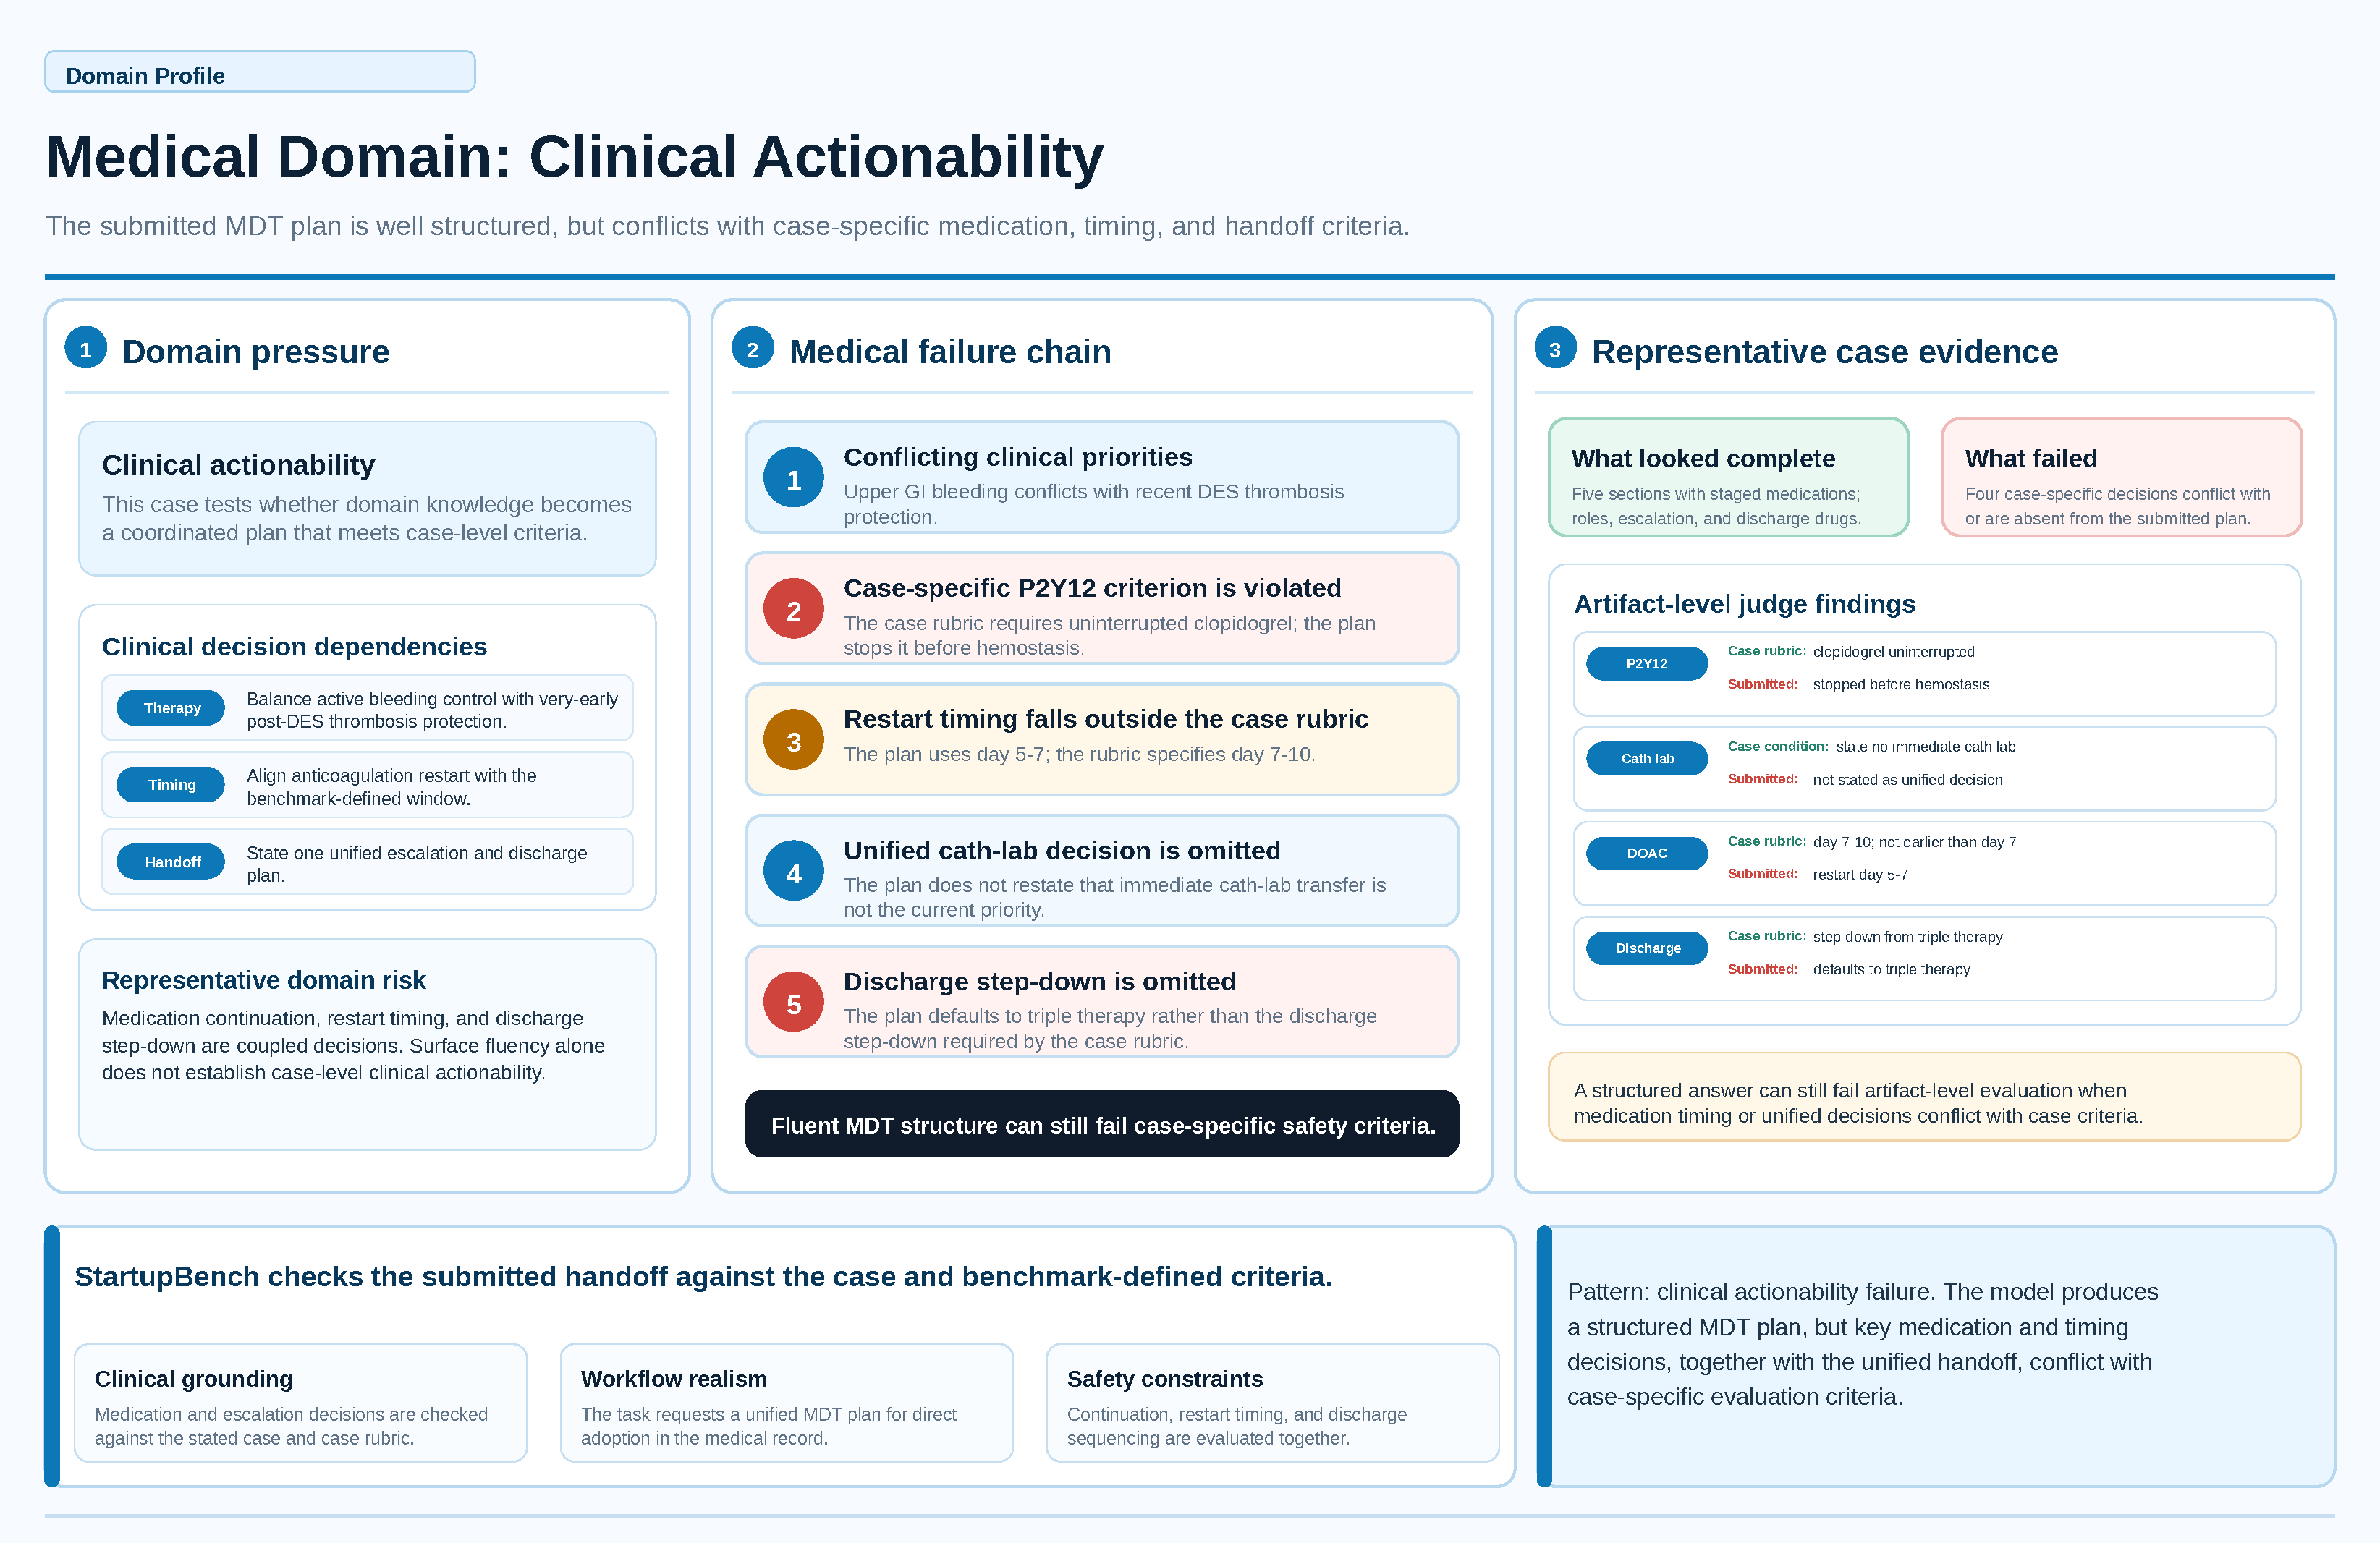
\includegraphics[width=0.99\textwidth]{figures/figure7_medical_clinical_actionability.pdf}
    \caption{
A representative example of failure caused by insufficient domain-specific clinical actionability.}
    \label{fig:domain-specify}
% \vspace{-6pt}
\end{figure*}
